\documentclass[10pt,twocolumn]{article}

% --- Minimal, Overleaf-friendly preamble (no exotic packages) --------------
\usepackage[margin=0.75in]{geometry}
\usepackage[T1]{fontenc}
\usepackage{lmodern}
\usepackage{microtype}
\usepackage{graphicx}
\usepackage{booktabs}
\usepackage{amsmath}
\usepackage{xcolor}
\usepackage{caption}
\usepackage[hidelinks]{hyperref}
\captionsetup{font=small,labelfont=bf}

% Put the PNGs from docs/assets/ next to this file (or in paper/figures/).
\graphicspath{{figures/}{../docs/assets/}}

\newcommand{\pc}{\%}  % readable percent in text

\title{\vspace{-2.5em}\textbf{Generalization and Evaluation Rigor in Deep\\
Reinforcement Learning: A From-Scratch Study on a\\
Financial-Market Testbed}}
\author{Daniel Lichtenberger\\
\small\texttt{github.com/Danny-397/RL-for-Crypto-and-stocks-}}
\date{\vspace{-1.2em}\small 2026}

\begin{document}
\maketitle

\begin{abstract}
\noindent Deep reinforcement learning is unusually easy to fool yourself with:
agents memorize their training trajectory, and a single lucky random seed can
masquerade as a real result. We study both failure modes from scratch --- a
PyTorch implementation of Proximal Policy Optimization (PPO), two custom
Gymnasium environments, and a full evaluation suite --- using financial markets
as a deliberately hard testbed: non-stationary, partially observable, with a
noisy reward and near--random-walk signal. We ask (RQ1) whether one fixed recipe
generalizes across two market regimes; (RQ2) how severely an agent overfits a
single price trajectory and whether \emph{domain randomization} repairs it;
(RQ3) whether an apparent out-of-sample edge survives multi-seed significance
testing; and (RQ4) whether the same holds for cross-sectional allocation. Our
headline result is negative, and that is the point: on real markets the agent
has \emph{no seed-robust edge} over buy-and-hold, and our own significance
tooling catches it: an earlier build of this study published a $+275\pc$
single-seed crypto run that survived neither reseeding nor a two-month extension
of the evaluation window. We further
introduce a \textbf{surrogate-data falsification test} that separates ``the agent
is weak'' from ``there is no signal to find,'' and validate it with a positive
control on synthetic data with known structure. In doing so the project
reproduces, in a new domain, the central methodological finding of
Henderson~et~al.\ (2018) --- that single-run RL evaluation is unreliable. We then
apply that finding to our own ablation: we report both arms as distributions over
ten seeds, where all four confidence intervals exclude zero, after finding and fixing
a seeding bug that had left the domain-randomized arm unreproducible. Finally (RQ5) we
turn the same PPO to a problem RL is suited to --- hedging a short option when trading
costs money --- where theory gives answers to check against. The agent approximately
recovers the Black-Scholes delta without observing it, learns to trade less as costs
rise, and on 237 real one-month SPY episodes it never trained on, ties a tuned
no-trade-band hedge at low costs and beats it at high costs. Last (RQ6), we put the
study through pre-registered checks from current deep-RL evaluation practice. They
find two real flaws: our PPO trails Stable-Baselines3 on two of four standard
benchmarks (seven implementation details close the gap on three of the four), and
the crypto split leaked across coins in calendar time. Neither changes the
conclusion: with the repaired PPO, Stable-Baselines3's PPO and SAC, at budgets up to
$10^6$ steps, on a leak-free split and on a stock universe chosen without hindsight,
no agent beats buy-and-hold.
\end{abstract}

\section{Introduction}
Reinforcement learning (RL) research has a reproducibility problem: reported
performance swings wildly across random seeds, implementation details, and
evaluation choices \cite{henderson2018}. Trading is a domain where these hazards
are especially acute --- the data-generating process drifts (non-stationarity),
price alone hides the true state (partial observability), the reward is noisy,
and a single historical path is trivial to memorize. That makes markets an
excellent \emph{stress test} for the general RL questions of generalization and
honest evaluation, rather than a get-rich scheme.

We build the entire stack from the algorithm up --- PPO \cite{ppo} with
Generalized Advantage Estimation \cite{gae}, two market environments, a
28-feature pipeline, and the evaluation harness --- so that every experiment can
be instrumented and trusted. Our contributions are:
\begin{itemize}\itemsep2pt
  \item A controlled study showing an RL agent memorizes a single price path
  catastrophically, and that \textbf{domain randomization}
  \cite{tobin2017,cobbe2019} is the single change that flips held-out return from
  reliably negative to reliably positive --- across ten seeds all four confidence
  intervals exclude zero, in both markets (\S\ref{sec:ablation}).
  \item A \textbf{multi-seed significance protocol} (bootstrap CIs + paired
  permutation tests) that reproduces the Henderson~et~al.\ \cite{henderson2018} finding in a new
  domain: a favorable single-seed ``win'' does not survive resampling
  (\S\ref{sec:sig}).
  \item An original \textbf{surrogate-data falsification test} that distinguishes
  agent weakness from signal absence, with a synthetic positive control that
  confirms the test has statistical power (\S\ref{sec:surrogate}).
  \item A \textbf{hedging study} in which the same PPO, trained only on simulated
  paths, is checked against two known answers (delta at zero cost, a widening
  no-trade band with costs) and then tested on real SPY history
  (\S\ref{sec:hedge}).
  \item A \textbf{pre-registered audit of the study itself} (\S\ref{sec:rigor}):
  the PPO benchmarked against a reference implementation, the trading result
  re-run with other implementations, another algorithm, larger budgets, a
  leak-free split and a hindsight-free universe, and every reported $p$-value
  corrected for multiple testing.
\end{itemize}

\section{Method}
\paragraph{Algorithm.} A single \texttt{PPOAgent} (shared-trunk actor--critic)
implements the clipped surrogate objective, GAE advantages, entropy
regularization, orthogonal initialization, gradient clipping, and a Welford
\cite{welford1962} running observation normalizer that is exported and reused at
serving time. A recurrent (LSTM) actor--critic trains through the same machinery
with truncated backpropagation through time.

\paragraph{Environments.} \texttt{StockTradingEnv} and \texttt{CryptoTradingEnv}
subclass one \texttt{BaseTradingEnv} so accounting, transaction costs, slippage,
and reward can never silently diverge. The action is a continuous target position
in $[-1,1]$ (fraction of equity; negative $=$ short). The observation is a rolling
window of 28 stationary features spanning multi-horizon momentum, moving-average
ratios, RSI/MACD, Bollinger \%B, Donchian position, ATR and volatility-regime
signals, drawdown-from-high, volume microstructure, and cross-asset context
(relative strength vs.\ SPY/BTC and the index's own trend).

\paragraph{Reward.} Two selectable forms: a risk-aware return net of transaction
costs with drawdown and turnover penalties, or the Differential Sharpe Ratio
\cite{moody2001}, an online per-step approximation to the change in the Sharpe
ratio.

\paragraph{Evaluation protocol.} Data are split chronologically; feature scalers
are fit on the training slice only. Agents are scored on an untouched test split
by total return, annualized Sharpe, and maximum drawdown, against buy-and-hold,
random, and moving-average-crossover baselines run through the identical cost
model. Every headline claim is repeated across independent seeds and reported as a
bootstrap 95\pc\ confidence interval, with a paired permutation test against
buy-and-hold.

\section{Experiments}

\subsection{RQ1: Regime transfer}
Holding the architecture and hyperparameters fixed, we train one agent per market
using only market-specific environment dynamics (cost, slippage, volatility). The
same recipe produces coherent, market-appropriate behavior on both equities and
crypto, confirming the unified agent is genuinely market-agnostic and that
downstream differences are attributable to the environments, not the code.

\subsection{RQ2: Overfitting and domain randomization}
\label{sec:ablation}
Training on a \emph{single} price series is a trap: the agent memorizes it. We
train two otherwise-identical agents --- one on a fixed synthetic path, one drawing
a fresh path every episode (domain randomization) --- and measure in-sample vs.\
out-of-sample (30 unseen paths) return (Table~\ref{tab:ablation}).

\begin{table}[t]\centering\footnotesize
\caption{Domain-randomization ablation, 10 seeds $\times$ 60k steps; all cells are
percent returns. Held-out is the mean over 30 unseen paths --- identical for every
arm and seed --- with a bootstrap 95\pc\ CI across seeds. In-sample is a
\emph{range} over seeds, not a mean: it is one leveraged compounding return on a
memorized path and spans orders of magnitude. The domain-randomized arm's in-sample
figure is its return on the very path the single-path agent memorized.}
\label{tab:ablation}
\setlength{\tabcolsep}{4pt}
\begin{tabular}{@{}llrr@{}}
\toprule
Market & Train & In-sample & Held-out [95\pc\ CI]\\
\midrule
% BEGIN GENERATED: tex-ablation
Stock  & single & $+6k$--$+31k$ & $-25$ {\scriptsize$[-33,-15]$}\\
Stock  & domain & $-22$--$+59$ & $\mathbf{+31}$ {\scriptsize$[+21,+44]$}\\
Crypto & single & $+87k$--$+4.0M$ & $-44$ {\scriptsize$[-59,-21]$}\\
Crypto & domain & $+24$--$+460$ & $\mathbf{+187}$ {\scriptsize$[+147,+229]$}\\
% END GENERATED: tex-ablation
\bottomrule
\end{tabular}
\end{table}

\begin{figure}[t]\centering
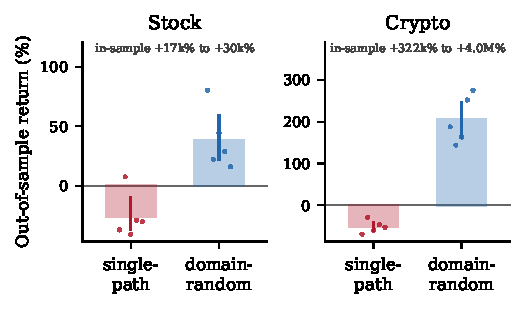
\includegraphics[width=\columnwidth]{fig_ablation}
\caption{Held-out return by training regime. Bars are the mean over seeds, whiskers
the bootstrap 95\pc\ CI, and dots the individual seeds --- so the reader sees $n$
and the spread rather than a bar alone. The in-sample range is annotated rather
than plotted: it spans several orders of magnitude and would flatten everything
else to a line.}
\label{fig:ablation}
\end{figure}

The astronomical in-sample figures are not a win --- they are the overfitting
signature. Domain randomization is the single change that turns a memorizer into a
generalizer, echoing sim-to-real transfer \cite{tobin2017} and RL generalization
benchmarks \cite{cobbe2019}.

Across ten seeds all four intervals exclude zero: single-path training is
reliably unprofitable out-of-sample and domain randomization is reliably
profitable, in both markets. The effect is therefore robust to seed choice, which
is the property the rest of this paper spends its time showing that real-market
edges lack.

Two caveats the distribution makes visible and a single run would hide.
``Reliably negative'' describes the mean, not every seed: in each market one of the
ten single-path seeds finished positive out-of-sample (stocks $+7.6\pc$, crypto
$+47\pc$), so a reader quoting any one run could have drawn the opposite
conclusion. The domain-randomized arm, by contrast, is positive in all twenty runs
(stocks $+11$ to $+80\pc$, crypto $+82$ to $+291\pc$), with no single seed carrying
the mean. Figure~\ref{fig:ablation} plots the individual seeds for exactly this
reason.

\subsection{RQ3: Does the edge survive multiple seeds?}
\label{sec:sig}
A single backtest is an anecdote. On synthetic markets where a signal provably
exists, the agent is repeatably profitable across 5 seeds --- its bootstrap
interval excludes zero in both markets --- yet remains statistically
indistinguishable from buy-and-hold under a paired permutation test. On
\emph{real} markets (Table~\ref{tab:real}; repaired PPO and leak-free split,
\S\ref{sec:rigor}) the agent is significantly \emph{worse} than buy-and-hold on
equities, and on crypto it loses money in every seed while remaining statistically
indistinguishable from a buy-and-hold that itself made little. In the previous
version of this study, whose crypto split leaked, the crypto mean was positive with
an interval above zero and the per-seed returns spanned $-29\pc$ to $+226\pc$: a
single run of either sign would have told a confident and wrong story. The paired test runs
across the held-out tickers, not across seeds. An earlier build of this study
(commit \texttt{d4c0ef9}) published the crypto agent at $+275\pc$ against
buy-and-hold's $+19\pc$; rebuilding the identical recipe --- same code, same seed,
same budget --- against a data snapshot pinned two months later erased that
headline entirely. The run was not merely seed-lucky but window-lucky.
Two later checks are in Table~\ref{tab:replication}. Re-running the same ten
seeds with identical code, budget and archived data on a different machine (same
PyTorch and NumPy) leaves the means within a point and the equity verdict unchanged,
but moves the crypto comparison across the 0.05 line: individual seeds diverge
across hardware, and six coins leave the paired test little margin. The crypto agent
is not better than buy-and-hold in either run; whether it is worse is not settled.
Adjusting for risk does not help it: its Sharpe ratio is below buy-and-hold's, and
regressed on the asset it traded, its alpha is negative in both markets, with a
crypto beta near zero that rules out ``short in a rising market'' as the explanation.

\begin{table}[t]\centering\small
\caption{Hardware replication and risk adjustment. Mean basket return and paired-test $p$ against buy-and-hold for the published run and a re-run of the same seeds (100--109) on a different machine; then, from the re-run, annualised Sharpe ratio (agent / buy-and-hold, paired test across tickers) and the agent's annualised alpha (sign-flip test against zero) and beta from regressing its daily returns on the traded asset's.}
\label{tab:replication}
\begin{tabular}{lrrrrr}
\toprule
Market & Published & Re-run & Sharpe & Alpha & Beta\\
\midrule
% BEGIN GENERATED: tex-replication
Stock  & $-26.5\pc$ ($p{=}0.0021$) & $-25.8\pc$ ($p{=}0.0021$) & $-0.53$ / $+1.12$ ($p{=}0.0021$) & $-12.6\pc$ ($p{=}0.0021$) & $0.14$\\
Crypto & $-44.6\pc$ ($p{=}0.22$) & $-45.4\pc$ ($p{=}0.03$) & $-0.61$ / $+0.32$ ($p{=}0.03$) & $-32.2\pc$ ($p{=}0.03$) & $0.00$\\
% END GENERATED: tex-replication
\bottomrule
\end{tabular}
\end{table}

\begin{table}[t]\centering\small
\caption{Real-market multi-seed significance (10 seeds, held-out walk-forward; $p$ from a paired permutation test across held-out tickers). Repaired PPO and one calendar cut for every ticker (\S\ref{sec:rigor}); seeds 100--109, 150k steps.}
\label{tab:real}
\begin{tabular}{@{}lrrl@{}}
\toprule
Market & Agent (95\pc\ CI) & vs.\ B\&H & Verdict\\
\midrule
% BEGIN GENERATED: tex-significance
Crypto & $-44.6\pc$ $[-56,-33]$ & $-55\pc$ & indist. ($p{=}0.2237$)\\
Stock  & $-26.5\pc$ $[-35,-17]$ & $-266\pc$ & worse ($p{=}0.0021$)\\
% END GENERATED: tex-significance
\bottomrule
\end{tabular}
\end{table}

This is exactly the warning of Henderson~et~al.\ \cite{henderson2018}: a single run is not evidence.
A naive project ships the lucky table; the significance test is what catches it.
\emph{Reporting the catch is the contribution.}

\subsection{RQ (original): A surrogate-data falsification test}
\label{sec:surrogate}
The results above show the agent does not beat the market --- but is that because
the agent is weak, or because there is no exploitable structure to find? We adapt
\textbf{surrogate-data testing} from nonlinear time-series analysis
\cite{theiler1992}. A \emph{return-shuffled surrogate} randomly permutes a series'
daily log-returns and re-integrates them. Because a sum is permutation-invariant,
the surrogate ends at the identical price --- \emph{buy-and-hold is unchanged} ---
but momentum, autocorrelation, and volatility clustering are destroyed. We then
train and evaluate the same recipe on structured data and on its surrogate and
compare the agent's edge over buy-and-hold.

The logic is a controlled falsification. On synthetic data with a \emph{known}
AR(1) momentum signal, a valid test must find $\text{edge}_{\text{structured}} \gg
\text{edge}_{\text{surrogate}}$: the agent should exploit the signal and lose that
edge once shuffling removes it. This is our positive control
(Table~\ref{tab:surrogate}), and it confirms the test has power. Applied to real
markets, the test finds \emph{no} significant difference between real and
return-shuffled data: on equities the agent does no better on real prices than on
structure-free surrogates ($\Delta$ nowhere near significant), the clean
null predicted by \S\ref{sec:sig}. The crypto arm is inconclusive --- heavy-tailed
returns produce occasional blow-ups on reshuffled paths that inflate the surrogate
loss and dominate the mean, and the gap is not significant; a median-based or
exposure-capped
statistic is the natural remedy. Neither market shows demonstrable exploited
structure, corroborating \S\ref{sec:sig} from a fresh angle and turning ``markets
are efficient'' from an appeal to authority into a falsifiable test.

\begin{table}[t]\centering\small
\caption{Surrogate-data test, synthetic positive control (edge $=$ agent $-$
buy-and-hold return, mean over 10 held-out paths, 5 seeds, 60k steps; $p$ from a
paired permutation test of structured vs.\ surrogate edge). When a known signal
exists the agent earns a positive edge; destroying it by shuffling collapses the
edge sharply negative --- the test has power in both markets.}
\label{tab:surrogate}
\begin{tabular}{@{}lrrrr@{}}
\toprule
Market & Structured & Surrogate & $\Delta$ & $p$\\
\midrule
% BEGIN GENERATED: tex-surrogate-control
Crypto & $+68.6\pc$ & $-55.7\pc$ & $+124.3\pc$ & $0.0075$\\
Stock  & $+1.8\pc$ & $-47.7\pc$ & $+49.5\pc$ & $0.0026$\\
% END GENERATED: tex-surrogate-control
\bottomrule
\end{tabular}
\end{table}

\subsection{RQ4: Cross-sectional allocation}
Single-asset timing is only half the problem. The same PPO agent generalizes to a
\texttt{PortfolioTradingEnv} that observes a whole basket and emits an
$N$-dimensional long/short weight vector under a gross-exposure budget, benchmarked
against an equal-weight ($1/N$) portfolio and a cross-sectional momentum factor. On
equities the learned allocator clears both random weights and the momentum factor
yet is beaten by equal-weight by more than 150 points of return; on crypto it is
level with random weights on return, ahead only on a risk-adjusted basis. The
contribution is the working, budget-constrained RL allocator and its
apples-to-apples evaluation --- the same lesson at a harder problem: naive
diversification is hard to beat when the per-asset signal is weak.

\subsection{RQ5: A decision problem where RL helps}\label{sec:hedge}
RQ1--RQ4 ask the agent to forecast; it cannot. Hedging is a decision problem whose
answer does not require a forecast. Sell one at-the-money call with 21 trading days
to expiry; each day choose a hedge $h\in[0,1]$ shares per option, paying a
proportional cost $c$ on the notional traded. A day's P\&L is
$h\,\Delta S-\Delta V-c\,|\Delta h|\,S$ with $V$ marked at Black-Scholes, and the
reward is $x-\tfrac12x^2$ for a P\&L of $x\pc$ of the notional, a mean-variance
objective \cite{kolm2019}. With $c=0$ the optimum is the Black-Scholes delta; with
$c>0$ it is a no-trade band around delta that widens with $c$ \cite{whalley1997}; in
general it has no closed form, which is where deep hedging \cite{buehler2019}
applies. The agent observes $\ln(S/K)$, time left, implied volatility and its own
hedge --- not delta --- and is trained only on simulated geometric-Brownian paths with
a fresh volatility per path (domain randomization, \S\ref{sec:ablation}), ten seeds
per cost. The strongest baseline is delta with a no-trade band whose width is tuned
per cost on separate validation paths. The real test uses 237 non-overlapping
one-month SPY episodes (2007--2026) with implied volatility $0.875\times$VIX.

\begin{table}[t]\centering\footnotesize
\caption{Hedging on real SPY history (higher score is better; median of 10 seeds).
Seeds beating the tuned band, with a paired permutation $p$ across seeds.}
\label{tab:hedge}
\begin{tabular}{@{}lrrrl@{}}
\toprule
Cost & Agent & Delta & Band & Seeds $>$ band\\
\midrule
% BEGIN GENERATED: tex-hedging
none & $-0.107$ & $-0.100$ & $-0.100$ & 4/10 ($p{=}0.315$)\\
0.05\pc & $-0.207$ & $-0.224$ & $-0.216$ & 7/10 ($p{=}0.805$)\\
0.2\pc & $-0.506$ & $-0.611$ & $-0.547$ & 9/10 ($p{=}0.006$)\\
1\pc & $-1.776$ & $-3.122$ & $-2.355$ & 10/10 ($p{=}0.002$)\\
% END GENERATED: tex-hedging
\bottomrule
\end{tabular}
\end{table}

Both checks are met in part or in full. At $c=0$ the agent's hedge stays within about
0.04 shares of delta and removes about 97\pc\ of the risk delta removes, but scores
below delta in all ten seeds: close, not exact. As $c$ rises its turnover falls and the
gap it tolerates to delta grows, a learned no-trade band. Against the tuned band
(Table~\ref{tab:hedge}) the agent ties at low costs and wins at 0.2\pc\ and 1\pc; in
simulation, where the band was tuned, the band wins below 1\pc. On real data the
agent's worst 5\pc\ of months are milder than the band's at every cost; we do not test
why. Prices are modelled, only the underlying is used to hedge, and rates and
dividends are omitted. A first check against real SPY option quotes finds the
volatility assumption close (at-the-money implied volatility $\approx 0.86\times$
VIX) and the zero-cost agents hedging one-day moves somewhat worse than delta, as in
simulation; full episodes on real quotes are accumulating and are reported in the
repository as they complete.

\subsection{RQ6: Does the study hold up?}\label{sec:rigor}
A negative result is only as good as the machinery behind it, so we applied to the
study the checks current practice asks of deep-RL results
\cite{henderson2018,agarwal2021}, each pre-registered with dated amendments before
its runs, on the replication's archived data and seeds 200--209.

\paragraph{Is the PPO correct?} Trained on four standard continuous-control tasks
with the trading study's own hyper-parameters, our PPO learns, but it is
significantly behind Stable-Baselines3 (SB3) \cite{sb3} configured identically on
HalfCheetah and Pendulum (Table~\ref{tab:bench}). No single change closes the gap;
seven standard implementation details \cite{huang2022} together do, on three of the
four tasks: a separate critic trunk; storing observations normalised as the policy
saw them (ours re-normalised them after the rollout with moved statistics, so each
update began from a ratio $\ne 1$); no tanh on the policy mean; bootstrapping
time-limit cut-offs; SB3's value loss; Adam $\epsilon=10^{-5}$; per-minibatch
advantage normalisation. Pendulum stays unexplained.

\begin{table}[t]\centering\footnotesize
\caption{Our PPO against Stable-Baselines3 under identical hyper-parameters (IQM of
final return, 10 seeds). $\downarrow$: significantly worse than SB3.}
\label{tab:bench}
\begin{tabular}{@{}lrrrr@{}}
\toprule
Task & Random & Ours & Repaired & SB3\\
\midrule
% BEGIN GENERATED: tex-rigor-bench
Pendulum-v1 & $-1{,}161$ & $-1{,}112^\downarrow$ & $-1{,}094^\downarrow$ & $-407$\\
InvertedPendulum-v5 & $5$ & $1{,}000$ & $1{,}000$ & $997$\\
HalfCheetah-v5 & $-292$ & $1{,}495^\downarrow$ & $4{,}176$ & $3{,}755$\\
Hopper-v5 & $17$ & $1{,}246$ & $1{,}499$ & $1{,}691$\\
% END GENERATED: tex-rigor-bench
\bottomrule
\end{tabular}
\end{table}

\paragraph{A calendar leak.} SAC's crypto result in the published design (+224\pc)
exposed a flaw: each coin was cut 60/40 on its own history, and crypto histories
start in different years, so ETH, ADA, XRP and SOL were trained through 15--27
months that are BTC's and LTC's test period. Cut on one calendar date, every
algorithm loses money on crypto (Table~\ref{tab:robust}). Every published crypto
number is inflated by the leak; stock series share their dates and are unaffected.

\begin{table}[t]\centering\footnotesize
\caption{Held-out basket return at 150k steps (IQM over seeds 200--209) by
implementation and algorithm (Rep.: repaired PPO; SB3: Stable-Baselines3 PPO;
leaky: the published per-coin split). On stocks every agent is significantly worse than
buy-and-hold ($p=0.002$); on the leak-free crypto split none is better.}
\label{tab:robust}
\begin{tabular}{@{}lrrrrr@{}}
\toprule
 & B\&H & Ours & Rep. & SB3 & SAC\\
\midrule
% BEGIN GENERATED: tex-rigor-trading
Stocks & $+240\pc$ & $-23\pc$ & $-30\pc$ & $-18\pc$ & $-25\pc$\\
Crypto, leaky & $+33\pc$ & $+13\pc$ & -- & $+28\pc$ & $+224\pc$\\
Crypto, leak-free & $+10\pc$ & $-29\pc$ & $-38\pc$ & $-64\pc$ & $-30\pc$\\
% END GENERATED: tex-rigor-trading
\bottomrule
\end{tabular}
\end{table}

\paragraph{Budget, universe, multiple testing.} Scored at seven budgets from 25k to
$10^6$ steps, no arm beats buy-and-hold at any of them. On the 30 Dow members of
2016-08-29, a universe chosen without hindsight, buy-and-hold falls from $+240\pc$
to $+101\pc$, and the agent still loses about a quarter of its capital and is
significantly worse than buy-and-hold. Of the fourteen $p$-values this paper
reports, every claim of a difference survives Holm--Bonferroni within its research
question; two (the hedging win at 0.2\pc\ cost and the crypto surrogate control)
do not survive one family of all fourteen.

\section{Related Work}
This project reproduces and cross-domain stress-tests results the field already
considers important. Henderson~et~al.\ \cite{henderson2018} document the unreliability of
single-run deep-RL evaluation; \S\ref{sec:sig} reproduces it on markets.
Tobin~et~al.\ \cite{tobin2017} introduce domain randomization for sim-to-real transfer and
Cobbe~et~al.\ \cite{cobbe2019} formalize train/test generalization in RL; \S\ref{sec:ablation}
measures the gap domain randomization closes. The algorithm is PPO \cite{ppo} with
GAE \cite{gae}; the Differential Sharpe Ratio reward is due to
Moody and Saffell \cite{moody2001}. The negative real-market result is consistent with weak-form
market efficiency \cite{fama1970}, and surrogate-data testing follows
Theiler~et~al.\ \cite{theiler1992}. The hedging study (\S\ref{sec:hedge}) follows deep
hedging \cite{buehler2019} and RL replication \cite{kolm2019}, and is checked against
the no-trade band of Whalley and Wilmott \cite{whalley1997}.

\section{Limitations and Conclusion}
The bottleneck is signal, not the agent: raw daily OHLCV carries little
exploitable structure, so richer exogenous data (macro series, sentiment) --- not a
bigger network --- is the natural next lever. A multi-fold walk-forward
(BTC-USD, 4 expanding-window folds $\times$ 5 seeds, on data through 2026-06-17) finds the agent losing money in
all four periods, pooled $-30.3\pc$ $[-43.9,-16.0]$; a head-to-head
feed-forward-vs-LSTM study is supported by the codebase and left as future work.

A second note concerns the ablation of \S\ref{sec:ablation}, because we found
the problem in our own results. The domain-randomized arm draws a fresh path every
episode --- that is what domain randomization means --- and in earlier builds that
stream was unseeded, so the run seed did not determine its data and no single run
of that arm could be reproduced. Both arms are now seeded (the path stream comes
from a per-seed factory), and a given seed reproduces its run exactly. Any
comparison that quotes one run of each arm would still not be a fair summary of
either.

This is why \S\ref{sec:ablation} reports each arm as a distribution over seeds
with bootstrap intervals, and why its conclusion is stated in terms of held-out
return --- a mean over 30 fixed evaluation paths --- rather than the single-path
in-sample figure, which averages nothing and compounds along one memorized
trajectory. Training additionally does not run under
\texttt{torch.use\_deterministic\_algorithms}, so exact bitwise reproducibility is
not guaranteed for either arm across machines. An earlier version of this table
quoted a single run per cell; that version was also stale with respect to a change
in the observation feature set, which is the ordinary way such numbers rot and an
argument for regenerating them from a script rather than transcribing them.

The audit of \S\ref{sec:rigor} adds two limitations of our own making: every
number in \S\S\ref{sec:sig}--\ref{sec:hedge} was produced by the published PPO,
which \S\ref{sec:rigor} shows was not equivalent to a reference implementation, and
the crypto rows used a split that leaked. Both were re-run for the central result
and did not change it; the remaining real-data crypto experiments have not been.

Our conclusion is deliberately unglamorous and, we argue, more
valuable than a suspicious backtest: built and evaluated honestly, a from-scratch
deep-RL trader finds no reliable edge on real markets --- and the methodology that
establishes this rigorously is the actual result. The same code is useful where
the problem is a decision with costs rather than a forecast: hedging an option, it
recovers what theory predicts and, on real prices, does better than the tuned
textbook rule where costs are high (\S\ref{sec:hedge}).

\begin{thebibliography}{15}\small
\bibitem{henderson2018} P.~Henderson, R.~Islam, P.~Bachman, J.~Pineau, D.~Precup,
  D.~Meger. Deep Reinforcement Learning that Matters. \emph{AAAI}, 2018.
\bibitem{ppo} J.~Schulman, F.~Wolski, P.~Dhariwal, A.~Radford, O.~Klimov.
  Proximal Policy Optimization Algorithms. \emph{arXiv:1707.06347}, 2017.
\bibitem{gae} J.~Schulman, P.~Moritz, S.~Levine, M.~Jordan, P.~Abbeel.
  High-Dimensional Continuous Control Using GAE. \emph{ICLR}, 2016.
\bibitem{tobin2017} J.~Tobin et al. Domain Randomization for Transferring Deep
  Neural Networks from Simulation to the Real World. \emph{IROS}, 2017.
\bibitem{cobbe2019} K.~Cobbe, O.~Klimov, C.~Hesse, T.~Kim, J.~Schulman.
  Quantifying Generalization in Reinforcement Learning. \emph{ICML}, 2019.
\bibitem{moody2001} J.~Moody, M.~Saffell. Learning to Trade via Direct
  Reinforcement. \emph{IEEE Trans.\ Neural Networks}, 2001.
\bibitem{theiler1992} J.~Theiler et al. Testing for Nonlinearity in Time Series:
  The Method of Surrogate Data. \emph{Physica D}, 1992.
\bibitem{fama1970} E.~Fama. Efficient Capital Markets. \emph{J.\ Finance}, 1970.
\bibitem{welford1962} B.~P.~Welford. Note on a Method for Calculating Corrected
  Sums of Squares and Products. \emph{Technometrics}, 1962.
\bibitem{buehler2019} H.~Buehler, L.~Gonon, J.~Teichmann, B.~Wood. Deep Hedging.
  \emph{Quantitative Finance}, 19(8), 2019.
\bibitem{kolm2019} P.~N.~Kolm, G.~Ritter. Dynamic Replication and Hedging: A
  Reinforcement Learning Approach. \emph{J.\ Financial Data Science}, 1(1), 2019.
\bibitem{whalley1997} A.~E.~Whalley, P.~Wilmott. An Asymptotic Analysis of an Optimal
  Hedging Model for Option Pricing with Transaction Costs. \emph{Mathematical
  Finance}, 7(3), 1997.
\bibitem{agarwal2021} R.~Agarwal, M.~Schwarzer, P.~S.~Castro, A.~Courville,
  M.~G.~Bellemare. Deep Reinforcement Learning at the Edge of the Statistical
  Precipice. \emph{NeurIPS}, 2021.
\bibitem{sb3} A.~Raffin, A.~Hill, A.~Gleave, A.~Kanervisto, M.~Ernestus,
  N.~Dormann. Stable-Baselines3: Reliable Reinforcement Learning Implementations.
  \emph{JMLR}, 22(268), 2021.
\bibitem{huang2022} S.~Huang, R.~F.~J.~Dossa, A.~Raffin, A.~Kanervisto, W.~Wang.
  The 37 Implementation Details of Proximal Policy Optimization. \emph{ICLR Blog
  Track}, 2022.
\end{thebibliography}

\end{document}
